\documentclass[11pt]{article}
\usepackage[utf8]{inputenc}
\usepackage{float}
\usepackage{amsmath}
\usepackage{tikz} % for Hasse diagram
\usepackage[hmargin=3cm,vmargin=6.0cm]{geometry}
%\topmargin=0cm
\topmargin=-2cm
\addtolength{\textheight}{6.5cm}
\addtolength{\textwidth}{2.0cm}
%\setlength{\leftmargin}{-5cm}
\setlength{\oddsidemargin}{0.0cm}
\setlength{\evensidemargin}{0.0cm}

\begin{document}
	
\section*{Student Information } 
%Write your full name and id number between the colon and newline
%Put one empty space character after colon and before newline
Full Name :  Can Erdogar \\
Id Number :  1942069 \\

% Write your answers below the section tags
\section*{Answer 1}
According to the handshaking theorem $2m = \sum_{v \in V} deg(v)$in a graph $G=(V,E)$ with m edges. \\
So, $46>4x$. Largest possible number of vertices is 11. \\

\section*{Answer 2}
Let's plug a new vertex into the G and connect this vertex with every other vertices in it. Then, the minimum degree of the vertices will increase to $\frac{n-1}{2} +1 =\frac{n+1}{2}$ which shows us that according to Dirac's theorem our new graph with n+1 vertices will have a hamilton circuit. When we remove the new vertex then we will get a hamilton path which proves your claim. \\

\section*{Answer 3}
According to the theorem 2 (in page 688 of the textbook) $\forall n A^{n}$ $(i,j)$ entry of $A^{n}$ will give the number of different paths of length n from $v_i$ to $v_j$ .  Because you can go back the same vertex in the bipartite graphs with even number of steps, diagonal entry of $A^{37}$ will be zero. \\

\section*{Answer 4}
\subsection*{a.}
\begin{table}[H]
\small
\centering
\caption{ Choice-Edge-Weight Kruskal }
\label{table:Kruskal}
\begin{tabular}{|c|c|c|}	%% specify column number
\hline 							%% line draw
1 & ${e,f}$& 1\\
\hline 
2 & ${e,h}$& 2\\
\hline 
3 & ${g,h}$& 2\\
\hline 
4 & ${a,d}$& 2\\
\hline 
5 & ${c,f}$& 3\\
\hline 
6 & ${d,g}$& 3\\
\hline 
7 & ${d,b}$& 3\\
\hline 
8 & ${h,i}$& 4\\
\end{tabular}
\end{table}

\subsection*{b.}
\begin{table}[H]
\small
\centering
\caption{ Choice-Edge-Weight Prim }
\label{table:Prim}
\begin{tabular}{|c|c|c|}	%% specify column number
\hline 							%% line draw
1 & ${e,f}$& 1\\
\hline 
2 & ${e,h}$& 2\\
\hline 
3 & ${g,h}$& 2\\
\hline 
4 & ${c,f}$& 3\\
\hline 
5 & ${d,g}$& 3\\
\hline 
6 & ${a,d}$& 2\\
\hline 
7 & ${d,b}$& 3\\
\hline 
8 & ${h,i}$& 4\\
\end{tabular}
\end{table}

\begin{figure}[H]	\caption{Delete the related edges to display the acquired MST}
	\centering
	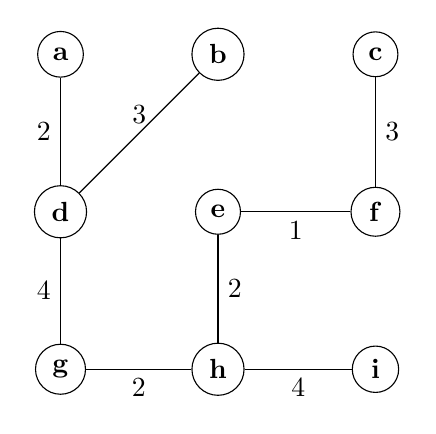
\begin{tikzpicture}
	
	\node[shape=circle,draw=black] (a) at (0, 4)     {\textbf{a}};
	\node[shape=circle,draw=black] (b) at (2, 4)     {\textbf{b}};
	\node[shape=circle,draw=black] (c) at (4, 4)     {\textbf{c}};
	\node[shape=circle,draw=black] (d) at (0, 2)     {\textbf{d}};
	\node[shape=circle,draw=black] (e) at (2, 2)     {\textbf{e}};
	\node[shape=circle,draw=black] (f) at (4, 2)     {\textbf{f}};
	\node[shape=circle,draw=black] (g) at (0, 0)     {\textbf{g}};
	\node[shape=circle,draw=black] (h) at (2, 0)     {\textbf{h}};
	\node[shape=circle,draw=black] (i) at (4, 0)     {\textbf{i}};
	
	
	\path[-] (a) edge  node[left]  {2} (d);
	\path[-] (b) edge  node[above] {3} (d);
	\path[-] (c) edge  node[right] {3} (f);
	\path[-] (d) edge  node[left]  {4} (g);
	\path[-] (e) edge  node[right] {2} (h);
	\path[-] (e) edge  node[below] {1} (f);
	\path[-] (g) edge  node[below] {2} (h);
	\path[-] (h) edge  node[below] {4} (i);
	
	\end{tikzpicture} 
\end{figure}

\end{document}